\documentclass{article}

\usepackage[english]{babel}
\usepackage{graphicx}
\usepackage{blindtext}

\usepackage[letterpaper,top=0.5cm,bottom=2cm,left=2cm,right=2cm,marginparwidth=1.75cm]{geometry}

\usepackage[colorlinks=true, allcolors=blue]{hyperref}

\begin{document}

\title {\textbf{Melanoma Detection with Deep Learning} \\[1ex] \large Science Depth Study}
\author{keyp0s}
\date{}
\maketitle

\subsection*{Introduction}

Skin cancer is the most prevalent type of cancer. Despite being the least frequent type of skin cancer, melanoma in particular is the cause of 75\% of skin cancer deaths. The American Cancer Society estimates over 100,000 new melanoma cases will be diagnosed in 2020. It's also expected that almost 7,000 people will die from the disease. As with other cancers, early and accurate detection can make treatment more effective.

\subsection*{Aim}

Dermatologists have a 67.4\% to 76.1\% of predicting melanoma based on clinical and dermoscopic images (Dermatology Practical & Conceptual, 2021). The goal of this experiment is to determine whether Deep Learning can predict melanoma with a higher accuracy than dermatologists.

\subsection*{Hypothesis}
The ResNet50 Deep Learning model will be able to predict melanoma in skin lesion images with a higher accuracy than dermatologists, due to the large training dataset and the complexity of the model.

\subsection*{Variables}
\begin{itemize}
\item[\textbf{-}] Independent Variable - Number of epochs used for training the model 
\item[\textbf{-}] Dependent Variable - Accuracy of melanoma prediction (on validation data)
\item[\textbf{-}] Control Variable - Accuracy of melanoma detection from human dermatologists 
\end{itemize}


\subsection*{Resources}
\raggedright The dataset used is the \href{https://www.nature.com/articles/sdata2018161}{HAM10k Dermatoscopic Image Collection from Harvard}. I used an augmented version that balanced the melanoma to non melanoma samples.
\linebreak

\begin{itemize}
\item[\textbf{-}] Link to augmented Kaggle version: \linebreak
\href{https://www.kaggle.com/datasets/drscarlat/melanoma}{https://www.kaggle.com/datasets/drscarlat/melanoma}
\linebreak

\item[\textbf{-}] Link to interactive notebook on Kaggle: \linebreak \href{https://www.kaggle.com/code/keypos/resnet50-melanoma-classification}{https://www.kaggle.com/code/keypos/resnet50-melanoma-classification}
\linebreak 

\item[\textbf{-}] Link to direct source code on github: \linebreak
\href{https://github.com/keyp0s/melanoma/blob/main/resnet50-melanoma-classification.ipynb}{https://github.com/keyp0s/melanoma/blob/main/resnet50-melanoma-classification.ipynb}
\end{itemize}

\subsection*{Method}
ResNet50 is being used as the base model. The model consists of 48 convolution layers which makes it exceptional at image recognition. The model is then trained on over 10,000 augmented images from the HAM10k dataset. These images will slowly train the model in a series of runs called epochs. In esence the model starts out with no prior knowledge and is fed one image at a time. At the beginning the predictions are almost random. When the model predicts an image wrong it takes that feedback and through back propagation adjusts its parameters. This is unfortunately a very complicated process  but at its core the model distinguishes features of melanoma lesions leading to the accuracy of the model exponentially increasing until it flattens off and peaks. This process will repeated for 16 epochs to avoid over-fitting on the data. A separate dataset of 3000 images the model has not been trained on will be used to test the models accuracy.
\linebreak

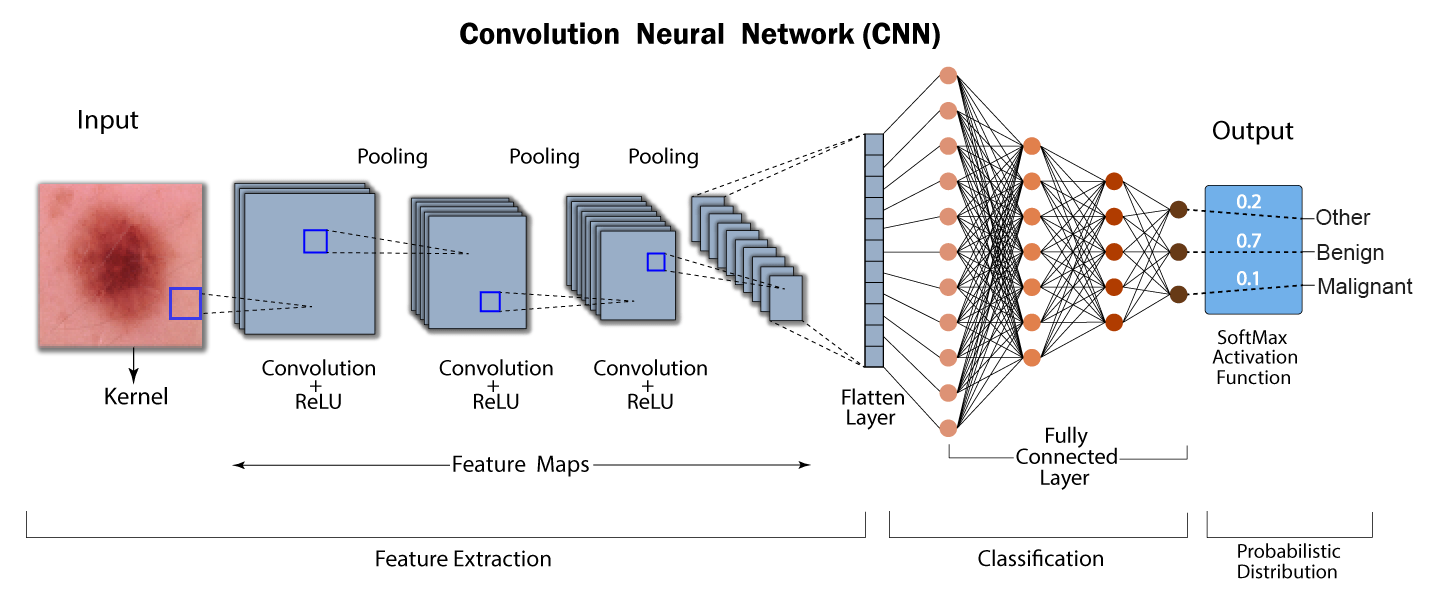
\includegraphics[width=7in]{cnn.png}
Figure 1: Example of Convolutional Neural Network Architecture
\subsection*{Results}
tbd

\subsection*{Discussion}

\subsection*{Bibliography}


\begin{itemize}
    \item[\textbf{-}] Kaggle. (2020). SIIM-ISIC Melanoma Classification \href{https://www.kaggle.com/competitions/siim-isic-melanoma-classification/overview}{https://www.kaggle.com/competitions/siim-isic-melanoma-classification/overview}
    \item[\textbf{-}]Organokov, M. (2021) SIIM-ISIC Melanoma Classification EfficientNet
    \href{https://www.kaggle.com/code/muhakabartay/siim-isic-melanoma-classification-efficientnet/notebook}{https://www.kaggle.com/code/muhakabartay/siim-isic-melanoma-classification-efficientnet/notebook}
    \item[\textbf{-}]Polesie, S., Jergéus, E., Gillstedt, M., Ceder, H., Dahlén Gyllencreutz, J., Fougelberg, J., Johansson Backman, E., Pakka, J., Zaar, O. and Paoli, J. (2021). Can Dermoscopy Be Used to Predict if a Melanoma Is In Situ or Invasive? Dermatology Practical & Conceptual
    \href{https://www.ncbi.nlm.nih.gov/pmc/articles/PMC8172039/}{https://www.ncbi.nlm.nih.gov/pmc/articles/PMC8172039/}
    \item[\textbf{-}]Tschandl, P., Rosendahl, C. and Kittler, H. (2018). The HAM10000 dataset, a large collection of multi-source dermatoscopic images of common pigmented skin lesions.
    \href{https://www.nature.com/articles/sdata2018161}{https://www.nature.com/articles/sdata2018161}
    \item[\textbf{-}]Tschandl, P. (2018). The HAM10000 dataset, a large collection of multi-source dermatoscopic images of common pigmented skin lesions.
    \href{https://dataverse.harvard.edu/dataset.xhtml?persistentId=doi:10.7910/DVN/DBW86T}{https://dataverse.harvard.edu/dataset.xhtml?persistentId=doi:10.7910/DVN/DBW86T}
    \item[\textbf{-}]Rasu, F., Dey, N. and Hashem, M. (2020). A Comparative Study of Neural Network Architectures for Lesion Segmentation and Melanoma Detection
    \href{https://www.researchgate.net/publication/342549085_A_Comparative_Study_of_Neural_Network_Architectures_for_Lesion_Segmentation_and_Melanoma_Detection}{https://www.researchgate.net/publication/342549085-A-Comparative-Study-of-Neural-Network-Architectures-for-Lesion-Segmentation-and-Melanoma-Detection}
\end{itemize}
\end{document}